\documentclass[11pt]{article}
\usepackage{bibentry}
\usepackage{url}
\usepackage[pdftex]{color,graphicx}
\usepackage{amsfonts}
\begin{document}
%\bibliographystyle{plain}
\nobibliography*

\title{ALF User Manual}
\author{Daniel A. Dalquen}
\maketitle

\section{Getting Started}
\subsection{Obtaining ALF}
ALF is available as a web service as well as a stand-alone version. Both are available at \url{http://www.alfsim.org}. The web service can be used to run simulations directly or to generate parameter files for the stand-alone version. I recommend using the web service only for small simulations. If you want to be notified when new releases are available, you can register with your email address, when you download the stand-alone version.

\subsection{Installing the stand-alone version}
When you download and unpack the stand-alone version of ALF, the following
files and directories are created:

\begin{description}
\item[\texttt{install.sh}] \hfill \\
install script (instructions below)
\item[\texttt{bin/}] \hfill \\
       - binaries of the darwin engine for Mac OS X and Linux\hfill \\
	   - starter scripts for darwin and ALF \hfill \\
	   - script to convert Fasta to Darwin files
\item[\texttt{lib/}] \hfill \\
       - the darwin library\hfill \\
	   - the entire ALF source code is located in lib/simulator
\item[\texttt{params/}] \hfill \\
sample parameter sets to reproduce some of the results from the publication
\end{description}

ALF can be started directly from this directory (see section \ref{sec.run}), but it will probably be more convenient to install the software, because that will allow you to start ALF directly from any directory.

To install ALF on your system, run the script install.sh. By default, binary and script files will be copied to \texttt{/usr/local/bin} and the \texttt{lib} directory will be copied to \texttt{/usr/local/share/alfdarwin} (this will require super user privileges). If you wish to install ALF in a different location, pass the path to that location as parameter to \texttt{install.sh}. For example, if you want to install ALF in your home directory, use
\begin{quote}
\texttt{./install.sh /path/to/home}.
\end{quote}
This will create the directories \texttt{bin/} and \texttt{share/alfdarwin/} in your home directory, if they don't exist already.

\subsection{Running Simulations}
\label{sec.run}
If you did not install ALF, run it with the following command:
\begin{quote}
\begin{verbatim}
bin/alfsim [path to parameter file]
\end{verbatim}
\end{quote}
If you did install ALF and the script is on your PATH, then this reduces to
\begin{quote}
\begin{verbatim}
alfsim [path to parameter file]
\end{verbatim}
\end{quote}

When no paramater file is given, ALF will look for the file parameters.drw in
the current working directory. Section \ref{sec.params} lists and explains all available parameters.

\subsection{Citing ALF}
If you use ALF in your research, please cite:
\begin{quote}
\bibentry{Dalquen:2011dx}
\end{quote}

\subsection{Contact information}
If you have a question or want to report a bug, please send
me an email to \url{d.dalquen@ucl.ac.uk}. 


\section{Parameters}
\label{sec.params}
Parameters for a simulation are passed in a parameter file that uses the Darwin syntax (see \url{http://www.biorecipes.com/DarwinHelp} for details). For example,
\begin{quote}
\texttt{protStart := 200;}
\end{quote}
sets the parameter \texttt{protStart} to 200. Note that each assignment is terminated by a semicolon.

Some parameters expect a list (comma-separated values enclosed in square brackets, e.g. \texttt{[2.4, 133.8]}) or a set (comma-separated values in curly brackets, e.g. \texttt{\{0, 1, 2.5\}}).

Strings are enclosed in single quotes, e.g. \texttt{'a string'}.

Finally, comments start with the number sign (\verb|#|).


\subsection{Tree Parameters}
ALF simulates sequences along a tree. This tree can be sampled randomly from a birth-death process or from a tree of life. Alternatively, you can also supply your own tree. The parameters below set up the species tree for the simulation.

\begin{itemize}
\item{\texttt{treeType}} \hfill \\
Method for creating the species tree. Accepts the following values:
\begin{description}
\item{\texttt{'BDTree'}} \hfill \\
Creates a birt-death tree with distance \texttt{mutRate} from origin to leaves, and $\lambda=\tt{birthRate}$ and $\mu=\tt{deathRate}$. Uses the sampling process described by \cite{Gernhard:2008p4607}.
\item{\texttt{'ToLSample'}} \hfill \\
Creates a tree by sampling from the tree of life (currently consists of 1038 species derived from OMA)
\item{\texttt{'Custom'}} \hfill \\
Use a custom tree defined by \texttt{treeFile}.
\end{description}
\item{\texttt{mutRate}} \hfill \\
Distance from origin to species at the leaves (for random trees)
\item{\texttt{scaleTree}} \hfill \\
Set to \texttt{true}, if the branch lengths of the tree should be scaled. When \texttt{treeLength} is defined as well, the sum of all branches will be scaled to match \texttt{treeLength}. Otherwise, the distance from root to deepest leaf is scaled to match \texttt{mutRate}. (default \texttt{false}).
\item{\texttt{treeLength}} \hfill \\
Sum of all branch lengths (only in conjunction with \texttt{scaleTree}).
\item{\texttt{birthRate}} \hfill \\
For \texttt{'BDTree'}: birth rate ($\lambda$)
\item{\texttt{deathRate}} \hfill \\
For \texttt{'BDTree'}: death rate ($\mu$)
\item{\texttt{NSpecies}} \hfill \\
The number of species in the tree (for \texttt{'BDTree'} and \texttt{'ToLSample'}).
\item{\texttt{ultrametric}} \hfill \\
For \texttt{BDTree}: should resulting tree be ultrametric (default \texttt{true}).
\item{\texttt{treeFile}} \hfill \\
String with path to tree file with tree in Darwin or Newick format. You can also directly assign a darwin tree structure, which has the following format:
\begin{quote}
\begin{verbatim}
Tree(Left,Height,Right,xtra)
\end{verbatim}
\end{quote}

\noindent where \texttt{Left} and \texttt{Right} can be another tree structure or a Leaf (\texttt{Leaf(Label, Height, xtra)}), \texttt{Height} is the distance of the node from the root and \texttt{extra} is a field for additional information (for example used to annotate the tree with model switches, see below).

\item{\texttt{unitIsPam}} \hfill \\
Set to \texttt{false} if branch lengths are in substitutions per site. Set rate parameters for events accordingly. By default, ALF uses PAM distances.
\end{itemize}

\subsection{Root Genome}
The genome at the root of the tree can either consist of your own sequences or can be randomly generated. The following parameters set up the root genome.
\begin{itemize}
\item{\texttt{realorganism}} \hfill \\
 A string specifying the path to the Darwin DB with the sequence data. Use the script \texttt{fasta2darwin} in the \texttt{bin} directory to convert Fasta files into the Darwin DB format.

\noindent \textbf{Example} (reads sequences from the file \texttt{se\_ECOLI\_core.db} in directory \texttt{realseed}):
\begin{quote}
\begin{verbatim}
realorganism := 'realseed/se_ECOLI_core.db';
\end{verbatim}
\end{quote}
\item{\texttt{protStart}} \hfill \\
The number of sequences that the first organism should have (only if the root genome is generated).
\item{\texttt{gammaLengthDist}} \hfill \\
List of parameters for the length distribution of the generated sequences ($\sim\Gamma(k,\theta)$). 

\noindent \textbf{Example} (lengths will be drawn from $\sim\Gamma(2.4,133.8)$):
\begin{quote}
\begin{verbatim}
gammaLengthDist := [2.4, 133.8];
\end{verbatim}
\end{quote}
If lengths of all sequences should be identical, set $k=\theta=1$ and specify the desired length with \texttt{minGeneLength}.

\item{\texttt{minGeneLength}} \hfill \\
Minimum length of a gene.
\end{itemize}

\subsection{Sequence types}
In ALF, you can configure different sequence types defined by a substitution model, an indel model and a model for rate variability among sites. The following sections describe how to set up the models, define sequence types and assign them to the sequences of the root genome. Switches between different sequence types can be performed during speciation or duplication.
 
\subsubsection{Substitution Models}
\label{sec.substmodels}
ALF supports a variety of nucleotide, codon and amino acid substitution models. Several models can be simulated in parallel for a subset of sequences. The parameters in this section allow you to set up substitution models.
\begin{itemize}
\item{\texttt{substModels}} \hfill \\
List of substitution models, where each model definition has the following format:
\begin{quote}
\begin{verbatim}
SubstitutionModel(name:string, parameters:list, 
                  frequencies:list, neutralDNA:boolean)
\end{verbatim}
\end{quote}
The number of arguments required depend on the model:
\begin{itemize}
\item models \texttt{CPAM}, \texttt{ECM}, \texttt{ECMu}, \texttt{GCB}, \texttt{JTT}, \texttt{WAG} and \texttt{LG} require just the name of the model (e.g. \texttt{SubstitutionModel('CPAM')}).
\item When using a custom matrix (\texttt{CustomC}, \texttt{CustomP}), pass the path to the matrix file as parameter.
\item For M-series models, pass also the codon frequencies (in the order AAA, AAC, AAG, AAT, ACA,\ldots, TTT).
\item Finally, for nucleotide models specify as fourth parameter whether non-sense mutations should be allowed.
\end{itemize}
Available models include:
\begin{description}
\item{nucleotide substitution} \hfill \\
\texttt{F84}, \texttt{GTR}, \texttt{HKY}, \texttt{TN93}
\item{codon substitution} \hfill \\
\texttt{CPAM}, \texttt{ECM}, \texttt{ECMu}, \texttt{M0}, \texttt{M2}, \texttt{M3}, \texttt{M8}, \texttt{CustomC}
\item{amino acid substitution} \hfill \\
\texttt{GCB}, \texttt{JTT}, \texttt{LG}, \texttt{WAG}, \texttt{CustomP}
\end{description}
Parameters are ordered as follows
\begin{description}
\item{custom empirical models} \hfill \\
\texttt{parameters[1]} should contain a path to a matrix in PAML format (lower triangular matrix of exchangabilitites, followed by a line with codon/aa frequencies).
\item{M-series models} \hfill \\
\texttt{parameters[1]}: $\kappa$ \hfill \\
\texttt{parameters[2]}: $\omega$ (single value or list) \hfill \\
\texttt{parameters[3]}: list of probabilities for $\omega$-class[es] \hfill \\
\texttt{parameters[4]}: for M8, parameter $p$ of beta distribution \hfill \\
\texttt{parameters[5]}: for M8, parameter $q$ of beta distribution \hfill \\
\item{nucleotide models} \hfill \\
\texttt{GTR}: \hfill \\
\texttt{parameters[1]}: $a$\hfill \\
\vdots \hfill \\
\texttt{parameters[6]}: $f$\hfill \\

\texttt{HKY}: \hfill \\
\texttt{parameters[1]}: $\alpha$ \hfill \\
\texttt{parameters[2]}: $\beta$ \hfill \\

\texttt{F84}: \hfill \\
\texttt{parameters[1]}: $\kappa$ \hfill \\
\texttt{parameters[2]}: $\beta$ \hfill \\

\texttt{TN93}: \hfill \\
\texttt{parameters[1]}: $\alpha_{1}$ \hfill \\
\texttt{parameters[2]}: $\alpha_{2}$ \hfill \\
\texttt{parameters[3]}: $\beta$ \hfill \\
\end{description}
\noindent \textbf{Example} (defines two substitution models, the CodonPam model for coding sequences and one a TN93 model with $\alpha_{1}=0.3, \alpha_{2}=0.4$ and $\beta=0.7$ and equal base frequencies for non-coding sequences):
\begin{quote}
\begin{verbatim}
substModels := [SubstitutionModel('CPAM'),
                SubstitutionModel('TN93', [.3, .4, .7],
                                  [seq(0.25,4)], true)]:
\end{verbatim}
\end{quote}

\item{\texttt{blocksize}} \hfill \\
When no substitution model is given (pure gap simulation), select block size for gaps
\end{itemize}

\subsubsection{GC Content Amelioration}
GC content amelioration can be enabled by setting the variable \texttt{targetFreqs}. There are three possibilities:
\begin{description}
\item{- \texttt{targetFreqs := ['Random'];}} \hfill \\
Creates random target frequencies for all leaf species and all models. Overrides frequencies supplied in substitution models.

\item{- Use specific frequencies per species and substitution model} \hfill \\
If you want to have specific target frequencies per species and substitution model, set \texttt{targetFreqs} to an array with the following structure:
\begin{quote}
\begin{verbatim}
targetFeqs := [freqsModel_1, freqsModel_2, ...]
\end{verbatim}
\end{quote}
where
\begin{quote}
\begin{verbatim}
freqsModel_i = [['speciesName_1', [freqList_1]],
                ['speciesName_2', [freqList_2]], ...]
\end{verbatim}
\end{quote}

\noindent \textbf{Example} (Simulation with 4 species using a single nucleotide model):
\begin{quote}
\begin{verbatim}
targetFreqs := [[['S1',[0.15, 0.35, 0.3, 0.2]],
                 ['S2',[0.2, 0.25, 0.3, 0.25]],
                 ['S3',[0.25, 0.2, 0.25, 0.3]],
                 ['S4',[0.35, 0.15, 0.2, 0.3]]]]:
\end{verbatim}
\end{quote}

\noindent \textbf{Note}: These target frequencies represent the stationary distribution of the underlying model. The actual frequencies will depend on the branch lengths.

\item{- Use different models} \hfill \\
You can define different substitution models for each branch (see section \ref{sec.substmodels}).
\end{description}

\subsubsection{Gap Models}
You can define multiple models for insertions and deletions and assign each of them (or have them assigned) to a subset of sequences. Use the following parameters to define indel models.
\begin{itemize}
\item{\texttt{indelModels}} \hfill \\
List of indel models, where each model definition has one of the following formats:
\begin{description}
\item{\texttt{IndelModel(0)}} \hfill \\
for no indels
\item{\texttt{IndelModel(rate:nonnegative, model:string, parameters:list, maxLen:posint)}} \hfill \\
for one model for insertions and deletions with the same rate
\item{\texttt{IndelModel(gainRate:nonnegative, model:string, parameters:list, maxLen:posint, lossRate:nonnegative)}} \hfill \\
for one model for insertions and deletions with separate rates for insertions and deletions
\item{\texttt{IndelModel(gainRrate:nonnegative, gainModel:string, gainParameters:list, gainMaxLen:posint, lossRate:nonnegative, lossModel:string, lossParameters:list, lossMaxLen:posint)}}\hfill \\
for separate models for insertions and deletions
\end{description}

\noindent The parameters are as follows:
\begin{itemize}
\item{\texttt{gainRate}/\texttt{lossRate}} \hfill \\
rate of insertions/deletions
\item \texttt{model} \hfill \\
can be one of the following:
\begin{description}
\item{\texttt{'ZIPF'}} \hfill \\
Use a Zipfian distribution of the form $L^{-\tt{Z\_c}}$, described in \cite{Chang:2004p3310}.
\item{\texttt{'NEGBIN'}} \hfill \\
Use a negative binomial distribution $\sim NB(\tt{NB\_r}, \tt{NB\_q})$
\item{\texttt{'QG'}} \hfill \\
Use the Qian-Goldstein distribution with parameters \texttt{QG\_c} and \texttt{QG\_t}, described in \cite{Qian:2001p3863}.
\item{\texttt{'GEOM'}} \hfill \\
Use a geometric distribution with parameter \texttt{E\_p}. This corresponds to a negative binomial distribution $\sim NB(1, \tt{E\_p})$
\item{\texttt{'CUSTOM'}} \hfill \\
Use a custom distribution with probabilities from \texttt{indelVector}.
\end{description}

\item{\texttt{gainParameters}/\texttt{lossParameters}} \hfill \\
the model parameters:
\begin{description}
\item{\texttt{'ZIPF'}} \hfill \\
\texttt{parameters[1]}: $c$ (Exponent of Zipfian distribution)
\item{\texttt{'GEOM'}} \hfill \\
\texttt{parameters[1]}: $p$ (geometric distribution with mean $1/p$)
\item{\texttt{'QG'}} \hfill \\
\texttt{parameters[1]}: $c$ \hfill \\
\texttt{parameters[2]}: $t$ (see \cite{Qian:2001p3863})
\item{\texttt{'NEGBIN'}} \hfill \\
\texttt{parameters[1]}: $r$ ($r \in \mathbb{N}$) \hfill \\
\texttt{parameters[2]}: $q$ ($0 < q < 1$)
\item{\texttt{'CUSTOM'}} \hfill \\
\texttt{parameters[1]}: $p_{1}$ ($\mathrm{Pr}(indel~of~length~1)$) \hfill \\
\vdots \hfill \\
\texttt{parameters[N]}: $p_{N}$ ($\mathrm{Pr}(indel~of~length~N)$) \hfill \\

A list with probabilities defining a custom indel distribution. Should be \texttt{MaxLen} elements long.
\end{description}

\item{\texttt{gainMaxLen}/\texttt{lossMaxLen}} \hfill \\
maximal length of indels
\end{itemize}
\item{\texttt{DawgPlacement}} \hfill \\
If \texttt{true} (default), each sequence is assumed to be part of a larger sequence and gaps can extend beyond either end of the sequence. This leads to a uniform distribution of gaps within the sequence. If \texttt{false}, gaps will be constrained to begin and end inside the sequence. This will lead to fewer gaps on both ends of the sequence.
\end{itemize}

\subsubsection{Rate Variation Among Sites}
The parameters in this section control rate variation among sites within sequences.
\begin{itemize}
\item{\texttt{rateVarModels}} \hfill \\
List of models for rate variation among sites. Each model definition has one of the following formats:
\begin{description}
\item{\texttt{RateVarModel()}} \hfill \\
for no rate variation
\item{\texttt{RateVarModel(model:string, areas:posint, motifFreq:nonnegative, alpha:nonnegative)}} \hfill \\
for defining a model
\end{description}

\noindent \textbf{Note}: These parameters are ignored, if M-series models or custom rates are used (use \texttt{RateVarModel()} in these cases).

\noindent The model definitions take the following parameters:
\begin{itemize}
\item{\texttt{model}} \hfill \\
possible values include:
\begin{description}
\item{\texttt{'None'}} \hfill \\
No rate variation among sites.
\item{\texttt{'Gamma'}} \hfill \\ % distribution of rates (Gamma or Poisson)
Use gamma rates. The number of bins is defined by \texttt{areas}, additionally, motifs occur with frequency \texttt{motifFreq}.
\item{\texttt{'Poisson'}} \hfill \\
Generates a random number of domains (at most \texttt{areas}) per gene with rates drawn from a Poisson distribution. \texttt{motifFreq} defines the fraction of domains with mutation rate 0 (motif).
\end{description}
\item{\texttt{areas}} \hfill \\
For \texttt{'Poisson'}: maximum number of areas with different rate within a gene. \hfill \\
For \texttt{'Gamma'}: number of rate classes. \hfill \\
\item{\texttt{motifFreq}} \hfill \\
Proportion of invariable sites (motifs)
\item{\texttt{alpha}} \hfill \\
Shape parameter of gamma distribution for gamma rates among sites.
\end{itemize}

\item{\texttt{areaPath}} \hfill \\
The path to a file, containing for each gene a list of areas with different substitution rates. The file should have the following format:
\begin{quote}
\begin{verbatim}
[areas_gene_1, areas_genes_2, ...]
\end{verbatim}
\end{quote}
\noindent where
\begin{quote}
\begin{verbatim}
areas_gene_i = [area_1, area_2, ...]
area_i = [start_pos, end_pos, rate]
\end{verbatim}
\end{quote}

\noindent \textbf{Note}: If you use \texttt{areaPath} to provide custom rate variation, set \texttt{rateVarModels} to \texttt{[RateVarModel()]} and define your sequence types (see section \ref{sec.seqtypes}) accordingly.
\end{itemize}

\subsubsection{Assigning and Switching Between Sequence Types}
\label{sec.seqtypes}
The following parameters define different sequence types and probabilities for switching between different types.
\begin{itemize}
\item{\texttt{seqTypes}} \hfill \\
A list of triplets \texttt{[i,j,k]}, where \texttt{i} defines the substitution model, \texttt{j} defines the indel model, and \texttt{k} defines the model for variation among sites.
\item{\texttt{seqTypeAssignments}} \hfill \\
Parameter concerning selection of sequence type for each sequence of the root genome. Either supply a list of frequencies of the types $1\ldots n$ defined in \texttt{seqTypes} for random assignment or a list of assignments for each sequence of the root genome.

\noindent \textbf{Example} (assign $T_{1}$ with probability $0.75$ and $T_{2}$ with probability $0.25$):
\begin{quote}
\begin{verbatim}
seqTypes := [[1,1,1], [2,1,1]];
seqTypeAssignments := [0.75, 0.25];
\end{verbatim}
\end{quote}
\item{\texttt{modelSwitchS}/\texttt{modelSwitchD}} \hfill \\
A matrix with probabilities for a switch from sequence type $T_{i}$ to type $T_{j}$ after speciation or duplication, respectively.

\noindent \textbf{Example} (switch from $T_{1}$ to $T_{2}$ with probability $0.2$ during speciation in the new species):
\begin{quote}
\begin{verbatim}
modelSwitchS := [[0.8,0.2],[0,1]];
modelSwitchD := [[1,0],[0,1]]; % no switch
\end{verbatim}
\end{quote}

\noindent \textbf{Note}: You can define model switches in more detail by using a custom tree and annotate it accordingly. Here is an example that creates the scenario depicted in figure \ref{fig.modelswitchtree} (branch lengths are 40 PAM for $a$ and $b$, and 80 PAM for $c$ - $f$):
\begin{quote}
\begin{verbatim}
treeFile := Tree(Tree(Leaf('S1', 120), 40, 
                      Leaf('S3', 120), [S,[[1,[3,4]]]]), 
                 0, Tree(Leaf('S2', 120), 40, 
                         Leaf('S4',120), [S,[[2,[5,6]]]]), 
                 [S,[[1,[1,2]]]]);
\end{verbatim}
\end{quote}

\begin{figure}[h!]
    \centering
    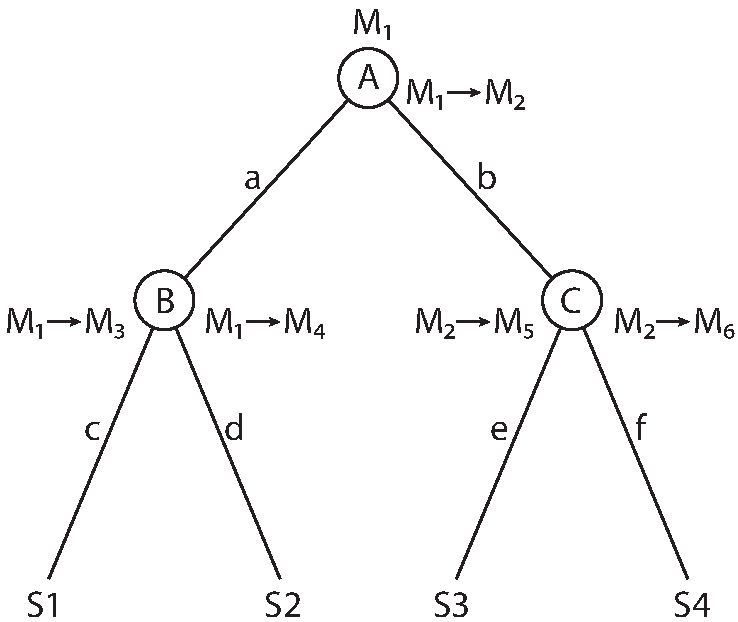
\includegraphics[width=0.5\textwidth]{modelswitchtree.pdf}
    \caption{This tree represents the following scenario: All sequences are initially assigned $T_{1}$. At node $A$, a switch occurs from $T_{1}$ to $T_{2}$ for branch $b$. At node $B$ a switch occurs from $T_{1}$ to $T_{3}$ for branch $c$ and from $T_{1}$ to $T_{4}$ for branch $d$. At node $C$ a switch occurs from $T_{2}$ to $T_{5}$ for branch $e$ and from $T_{2}$ to $T_{6}$ for branch $f$.}
    \label{fig.modelswitchtree}
\end{figure}
\end{itemize}

\subsection{Rate Variation Among Genes}
The parameters in this section control rate variation among sequences.
\begin{itemize}
\item{\texttt{amongGeneDistr}} \hfill \\
Distribution of rates among genes. Possible values include:
\begin{description}
\item{\texttt{'None'}} \hfill \\
No variation among genes.
\item{\texttt{'Gamma'}} \hfill \\
Draw rate for each sequence from a gamma distribution with shape parameter \texttt{aGAlpha} and average $1$.
\item{\texttt{'Custom'}} \hfill \\
Use custom rates from file defined by \texttt{aGPath}.
\end{description}
\item{\texttt{aGAlpha}} \hfill \\
Shape parameter of among gene rate distribution.
\item{\texttt{aGPath}} \hfill \\
Path to file with custom rates (see example file, only for custom root sequences)
\end{itemize}


\subsection{Gene Duplication and Loss}
The following parameters control gene duplication and gene loss.
\begin{itemize}
\item{\texttt{geneDuplRate}} \hfill \\
Rate of gene duplications (relative to substitutions).
\item{\texttt{transDupl}} \hfill \\
Probability of a tranlocation after duplication.
\item{\texttt{numberDupl}} \hfill \\
Maximum number of consecutive genes involved in one duplication event.
\item{\texttt{fissionDupl}} \hfill \\
Probability of a fission event after the duplication of a single gene.
\item{\texttt{fusionDupl}} \hfill \\
Probability of a fusion event after the duplication of two or more genes.
\item{\texttt{P\_pseudogene}} \hfill \\
Probability of duplicate becoming a pseudogene (permanent rate change for duplicate).
\item{\texttt{ratefac\_pseudogene}} \hfill \\
Factor by which the rate for the pseudogene is modified.
%%% duplicate evolves under neofunctionalization 
\item{\texttt{P\_neofunc}} \hfill \\
Probability of duplicate undergoing neofunctionalization (temporary rate change for duplicate).
\item{\texttt{ratefac\_neofunc}} \hfill \\
Factor by which the rate for the duplicate is modified.
\item{\texttt{life\_neofunc}} \hfill \\
Life of increased rate (time to normalization of rate, in PAM units or substitutions per site)
%%% both copies evolving by subfunctionalization 
\item{\texttt{P\_subfunc}} \hfill \\
Probability of both copies undergoing subfunctionalization (temporary rate change for original and duplicate)
\item{\texttt{ratefac\_subfunc}} \hfill \\
Factor by which the rate for the duplicate is modified.
\item{\texttt{life\_subfunc}} \hfill \\
Life of rate change (time to normalization of rate, in PAM units or substitutions per site).
  
\item{\texttt{geneLossRate}} \hfill \\
Rate of gene losses (relative to substitutions)
\item{\texttt{numberLoss}} \hfill \\
Maximum number of consecutive genes involved in one loss event.
\end{itemize}

\subsection{Lateral Gene Transfer}
\begin{itemize}
\item{\texttt{lgtRate}} \hfill \\
Rate of single lateral gene transfers (relative to substitutions).
\item{\texttt{orthRep}} \hfill \\
Proportion of lateral gene transfers that are orthologous replacements (i.e. the transferred gene replaces the orthologous gene in the recipient).
\item{\texttt{lgtGRate}} \hfill \\
Rate of lateral transfers of groups of genes.
\item{\texttt{lgtGSize}} \hfill \\
Maximum number of genes which can be transferred in one event.
\end{itemize}

\subsection{Genome Rearrangement}  
\begin{itemize}
\item{\texttt{invers}} \hfill \\
Rate of gene inversions (relative to substitutions).
\item{\texttt{invSize}} \hfill \\
Maximum number of genes which are inverted in one inversion event
\item{\texttt{transloc}} \hfill \\
Rate of gene translocations (relative to substitutions).
\item{\texttt{transSize}} \hfill \\
Maximum number of genes which are translocated in one go
\item{\texttt{invtrans}} \hfill \\
Rate of inverted translocations (relative to substitutions).
\end{itemize}

\subsection{Gene Fusion and Fission}
\begin{itemize}
\item{\texttt{fissionRate}} \hfill \\
Rate of gene fissions without prior duplication (relative to substitutions).
\item{\texttt{fusionRate}} \hfill \\
Rate of gene fusions without prior duplication of fused genes (relative to substitutions).
\item{\texttt{numberFusion}} \hfill \\
Maximum number of genes fused in one event.
\end{itemize}

\subsection{Output}
The following parameters define what output is generated and where it is stored. ALF will always generate a species tree, that reflects the ancestry of the simulated species, and the set of genomes of the species at the leaves of that tree.

\begin{itemize}
\item{\texttt{simOutput}} \hfill \\
A set of output files and formats. If this variable is not defined, all outputs are generated. Possible values include:
\begin{description}
\item{\texttt{'GeneTrees'}}\hfill \\
all gene trees
\item{\texttt{'Ancestral'}}\hfill \\
output ancestral genomes
\item{\texttt{'Dup'}}\hfil \\
output ancestral sequences at gene duplications. The output consists of one file per species. Each sequence is only 
stored in one file (i.e. the one of the species where the duplication occurred).
\item{\texttt{'MSA'}}\hfill \\
MSAs of all related sequences
\item{\texttt{'VP'}}\hfill \\
pairwise evolutionary relationships (ortho/para/xenologs)
\item{\texttt{'DarwinTree'}}\hfill \\
output trees in Darwin format
\item{\texttt{'Newick'}}\hfill \\
output trees in Newick format (default)
\item{\texttt{'DarwinDB'}}\hfill \\
output genomes as Darwin databases
\item{\texttt{'Fasta'}}\hfill \\
output genomes as Fasta files (default)
\end{description}

\noindent \textbf{Example} (creates species tree in Darwin format, MSAs of all gene families, and Darwin databases for all ancestral and leaf species):
\begin{quote}
\begin{verbatim}
simOutput := {'DarwinTree', 'MSA', 'DarwinDB', 'Ancestral'};
\end{verbatim}
\end{quote}

\item{\texttt{wdir}} \hfill \\
A string specifying the working directory, i.e. the directory where simulation results are stored. current working directory by default, can also be set as argument of alfsim

\item{\texttt{mname}} \hfill \\
A string specifying the name of the simulation. ALF will create a directory of that name in the working directory containing all result files.
\end{itemize}

\subsection{Misc}
\begin{itemize}
\item{Initialize random number generator} \hfill \\
If you are interested in getting reproducible results, put \texttt{SetRand(}$seed$\texttt{);} on the very first line of the parameter file, where $seed$ is an arbitrary integer number.
\end{itemize}

\section{The Evolutionary History of a Gene}
The Darwin database files hold information about all evolutionary events that affected a gene. For each gene, the \texttt{<DE>} tag contains a string composed of the following elements:
\begin{itemize}
\item{\texttt{a-(x)b}} speciation at time x of species a into species b
\item{\texttt{-(gDx)a}} gene duplication of gene g at time x in species a
\item{\texttt{-a(gLx)b}} LGT (novel acquisition) of gene g at time x from donor species a into recipient species b
\item{\texttt{-a(gLox)b}} LGT (orthologous replacement) of gene g at time x from donor species into recipient species b
\item{\texttt{-(gFix)a}} gene fission of gene g at time x in species a
\item{\texttt{-(gFux)a}} gene fusion of gene g with the current gene at time x in species a
\end{itemize}

\section{Performance / Memory Usage}
%Table \ref{tab.performance} lists execution time and memory usage for a number of example simulations.

\begin{table}[htp]
\begin{center}
\begin{footnotesize}
\begin{tabular}{lcc}
\hline
\bf{Simulation}            & \parbox{2cm}{\bf{Execution Time (s)}}        & \parbox{2.0cm}{\bf{Memory\\ Usage (MB)}} \\
\hline
\parbox{7.3cm}{root genome: 100 protein sequences, 500 aa each; 20 species; substitutions: WAG} & 7 & 300 \\
\hline
\parbox{7.3cm}{root genome: 100 protein sequences, 500 aa each; 20 species; substitutions: WAG; indels: Zipfian; $\Gamma$ rates} & 10 & 664 \\
\hline
\parbox{7.3cm}{root genome: 100 codon sequences, 500 codons each; 20 species; substitutions: CPAM; indels: Zipfian; $\Gamma$ rates} & 315 & 1506 \\
\hline
\parbox{7.3cm}{root genome: 100 codon sequences, 500 codons each; 20 species; substitutions: CPAM; indels: Zipfian; $\Gamma$ rates; duplications/losses with rate 0.001} & 277 & 1489 \\
\hline
\parbox{7.3cm}{root genome: 1000 seqs, lengths $\sim\Gamma(3,134)$; 20 species; substitutions: CPAM, TN93; indels: Zipfian; $\Gamma$-rates; duplications/losses/fusions/fissions with rate 0.001; LGTs with rate 0.0004; rearrangements with rate 0.005} & 1782 & 1801 \\
\hline
\parbox{7.3cm}{root genome: 4352 E. coli genes; 20 species; substitutions: CPAM, TN93; indels: Zipfian; $\Gamma$-rates; duplications/losses with rate 0.003; LGTs with rate 0.0005} & 16577 & 3934 \\

\hline
\end{tabular}
\end{footnotesize} % small
\end{center}
\caption{Performance of a number of example simulations. Based on simulations run on a Indel Core 2 Quad with 2.33 GHz.}
\label{tab.performance}
\end{table}


\bibliographystyle{plain}
\bibliography{manual}

\end{document}
